\documentclass{beamer}

\usepackage{amsmath}
\usepackage{amssymb}
\usepackage{booktabs}
\usepackage{epstopdf} %converting to PDF

\usetheme{AnnArbor}
\usecolortheme{beaver}

\mode<presentation>

\title{Overview of Results from Reggio}
%\author{P. Biroli et al.}
\date{\today}

\begin{document}

% Title Page
\begin{frame}
	\titlepage
\end{frame}

%\begin{frame}
%	\tableofcontents
%\end{frame}

\section{Data}
\subsection{Sample}

%%%%%%%%%%

\begin{frame}
	\frametitle{Cohort Structure}
	\begin{itemize}
	\item In each of the three cities (Reggio Emilia, Parma, and Padova), individuals in the following cohorts were interviewed.
	\end{itemize}
	\centering
	\vspace{1cm}
	\begin{tabular}{ccc}
	\toprule
	Cohort & Birth Year(s) & Age at Interview \\
	\midrule
	I & 1954-1959 & 54-60 years old  \\
	II & 1969-1971 & 43 years old \\
	III & 1981-1981 & 32 years old \\
	IV & 1994 & last year of compulsory schooling  \\
	V & 2006 & 1st year of elementary school  \\
	\bottomrule
	\end{tabular}
\end{frame}

%%%%%%%%%%

\begin{frame}
	\frametitle{Treatment and Control Structure}
\footnotesize Currently, this is the treatment and control structure, according to participation to Reggio Children preschool. Cohort I was born before the start of the Reggio program.

	\vspace{0.2cm}
	\centering
	\footnotesize
	\begin{tabular}{ccccc}
	\toprule
	Cohort & \multicolumn{4}{c}{City} \\
	 & \multicolumn{2}{c}{Reggio} & Parma & Padova \\
	 & Municipal & Other & All & All \\
	\midrule
	I &  & C & C & C \\
	& & 200 & 103 & 146 \\
	II & T & C & C & C \\
	& 125 & 160 & 254 & 252 \\
	III & T & C & C & C \\
	& 143 & 137 & 251 & 251 \\
	IV & T & C & C & C \\
	& 156 & 144 & 254 & 282 \\
	V Ita. & T & C & C & C \\
	& 160 & 151 & 291 & 278 \\
	V Imm. & T & C & C & C \\
	&  70 &  40 &  58 & 113 \\
	\bottomrule
	\end{tabular}

\hyperlink{tab:RespRate}{\beamergotobutton{Response rate}}
\end{frame}

%%%%%%%%%%	

\begin{frame}
	\frametitle{Cohort Aggregation}
	\begin{itemize}
		\item For this preliminary analysis, the cohorts will be aggregated into:
		\begin{itemize}
			\item Child (Cohort V)
			\item Adolescent (Cohort IV)
			\item Adult (Cohorts I, II, III)
		\end{itemize}
	\end{itemize}
\end{frame}

%%%%%%%%%%	

\subsection{Variables for Analysis}

\begin{frame}
	\frametitle{Outcomes}
	To begin, we present results for the following outcomes:
	\begin{itemize}
		\item Strengths and Difficulties Questionnaire (SDQ) 
		\item Depression Scale (CESD)
		\item In good health
		\item Negative attitudes towards migrants
	\end{itemize}
\vspace{2ex}
\begin{footnotesize}
These variables were chosen to 
\begin{itemize}
 	\item Represent different domains (noncog skills, physical health, preferences)
 	\item Span all the cohorts
 	\item Show preliminary results for both continuous and dummy outcomes
 	\vspace{2ex}
 	\item[$\hookrightarrow$] Additional outcomes will be analyzed once the identification procedure has been refined
\end{itemize}
\end{footnotesize}
\end{frame}

%%%%%%%%%%

\begin{frame}
	\frametitle{Outcome Availability by Age Group}
	\centering
	\begin{tabular}{cccc}
	\toprule
	Outcome & \multicolumn{3}{c}{Age Group} \\ 
	\cmidrule{2-4}
	& Child & Adolescent & Adult \\
	\midrule
	Caregiver-reported SDQ & $\checkmark$ & $\checkmark$&  \\
%	Individual-reported SDQ &  & $\checkmark$ &  \\
	\cmidrule{1-1}
	Caregiver-reported good health & $\checkmark$ & $\checkmark$ &  \\
	Individual-reported good health &  & & $\checkmark$ \\ %$\checkmark$ for adolescent taken away
	\cmidrule{1-1}
	Depression &  & $\checkmark$ & $\checkmark$ \\
	\cmidrule{1-1}
	attitudes vs. migrants & & $\checkmark$& $\checkmark$ \\
	\bottomrule
	\end{tabular}
\end{frame}

%%%%%%%%%%

\section{Analysis: Raw Data}
\begin{frame}\frametitle{Raw means}
The following plots show raw-averages and standard error of the variables of interest.
\begin{itemize}
	\item They are split by city and preschool type.
	\vspace{2ex}
	\begin{small}
	\item Num of obs. in each cell is reported on the bottom of the graph
	\item Cells with less than 5 obs are omitted
	\end{small}
\end{itemize}
\end{frame}

%%%%%%%%%%%% SDQ %%%%%%%%%%%%%%%%%%%
\begin{frame}
\begin{itemize}
	\centering
	\item[1.] Strength and Difficulties Questionnaire
	\begin{itemize}
		\centering
		\item Raw score, ranging from 0 to 40
		\item Higher score indicates more difficulties
	\end{itemize}
\end{itemize}
\end{frame}

\begin{frame}
\center
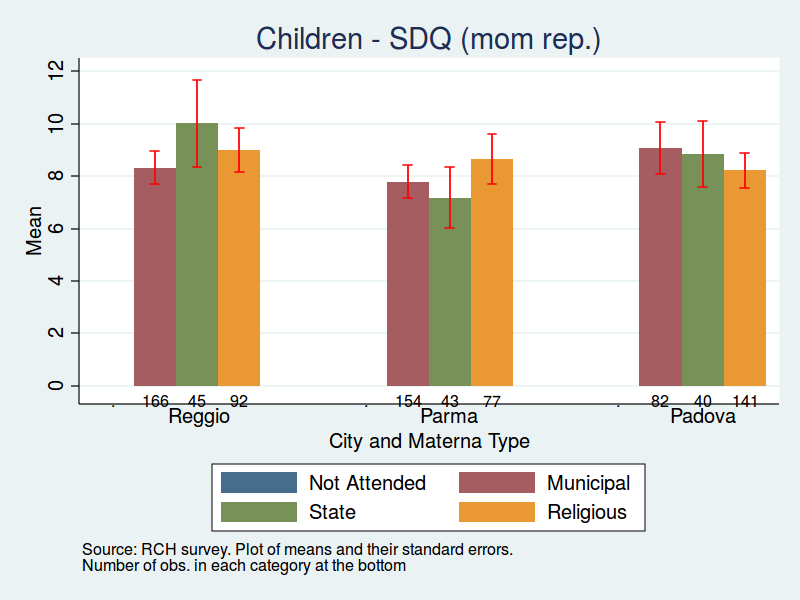
\includegraphics[scale=0.40]{../Output/childSDQ_score_Child.png}
\end{frame}

\begin{frame}
\center
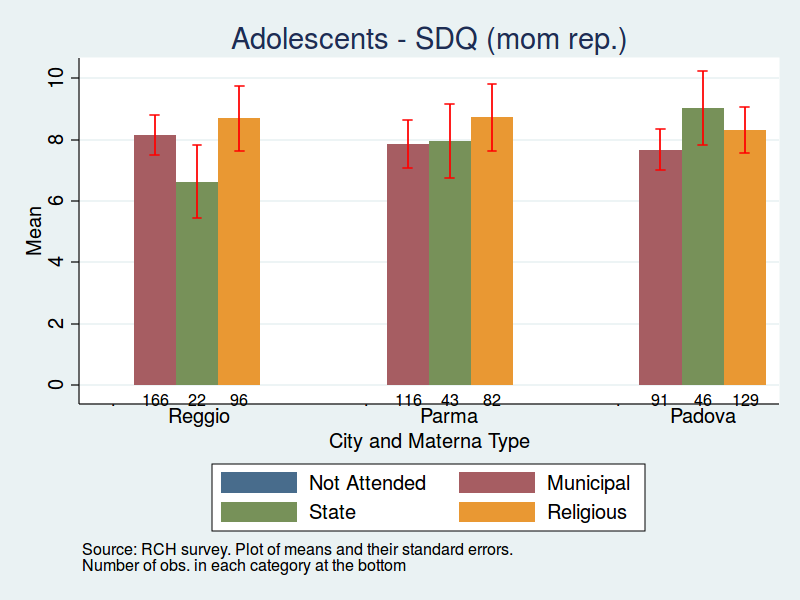
\includegraphics[scale=0.40]{../Output/childSDQ_score_Ado.png}
\end{frame}

%\begin{frame}
%\center
%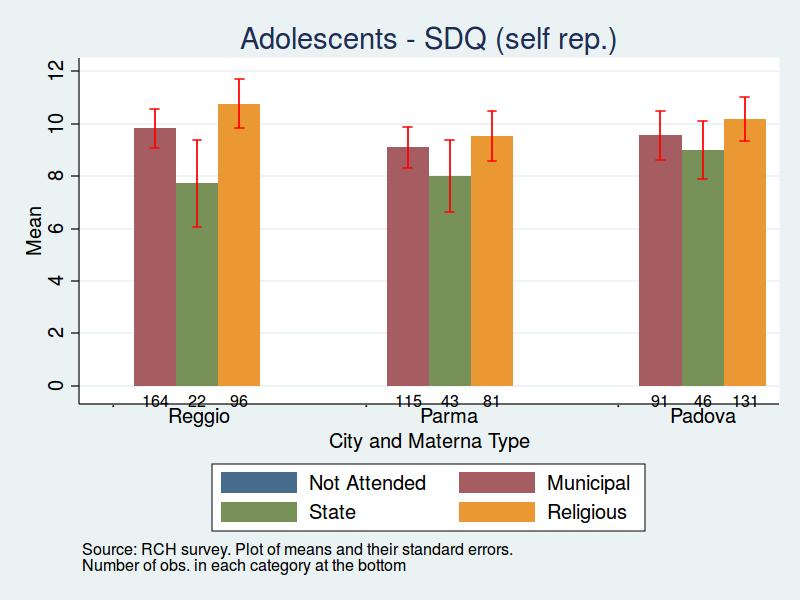
\includegraphics[scale=0.40]{../Output/SDQ_score_Ado.png}
%\end{frame}

%%%%%%%%%%%% Depression %%%%%%%%%%%%%%%%%%%
\begin{frame}
\begin{itemize}
	\centering
	\item[2.] Depression CES-D scale
	\begin{itemize}
		\centering
		\item Raw score, ranging from 10 to 50
		\item Higher score indicates more depressive symptoms 
	\end{itemize}
\end{itemize}
\end{frame}

\begin{frame}
\center
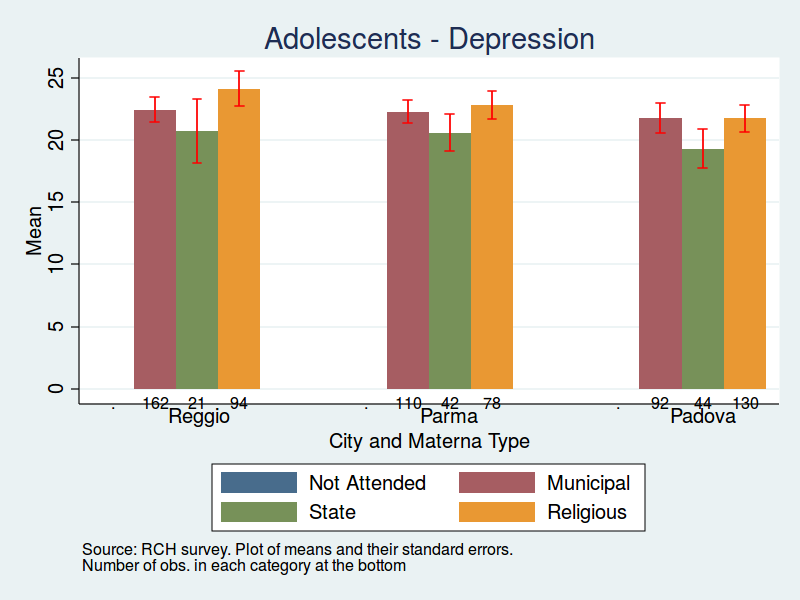
\includegraphics[scale=0.40]{../Output/Depression_score_Ado.png}
\end{frame}

\begin{frame}
\center
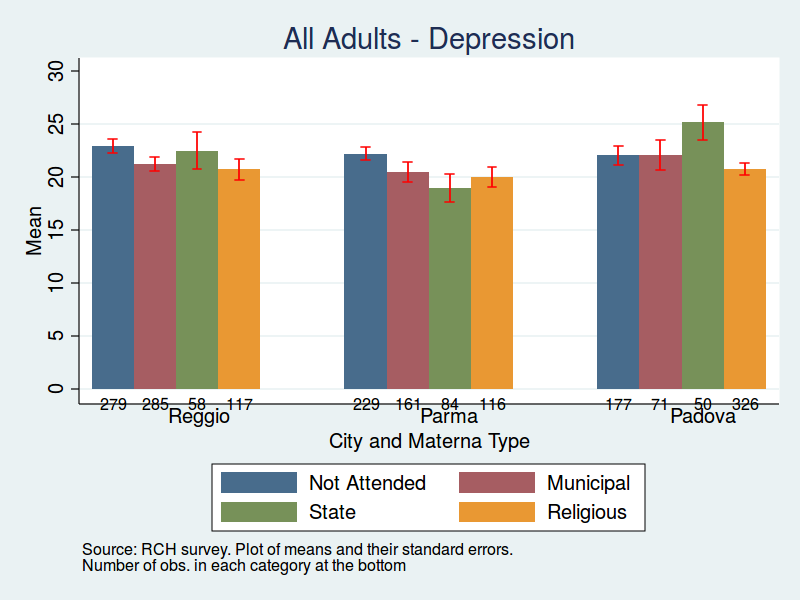
\includegraphics[scale=0.40]{../Output/Depression_score_AllAdults.png}
\end{frame}

%%%%%%%%%%%% Health %%%%%%%%%%%%%%%%%%%
\begin{frame}
\begin{itemize}
	\centering
	\item[3.] In good health
	\begin{itemize}
		\centering
		\item Responded `excellent' or `good' to the question ``in general, how would you describe your (your child's) health?'' (5-point likert scale)
	\end{itemize}
\end{itemize}
\end{frame}

\begin{frame}
\center
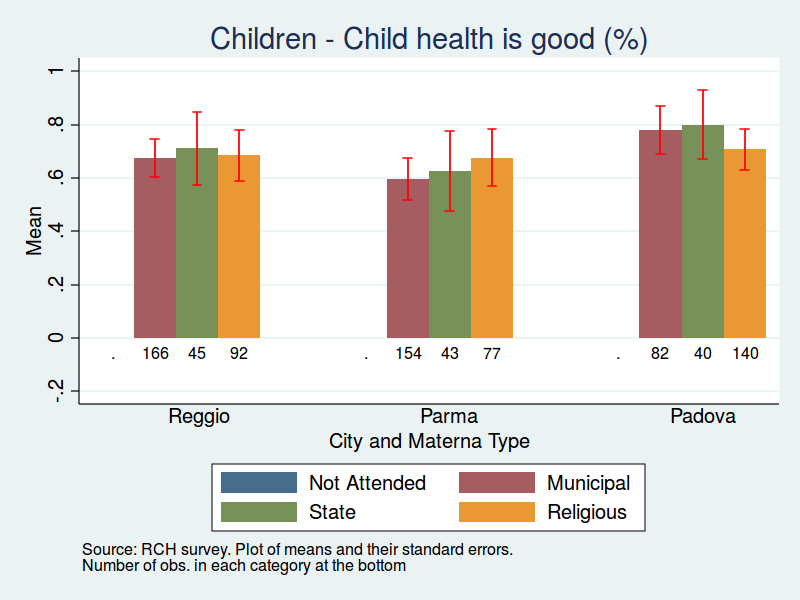
\includegraphics[scale=0.40]{../Output/childHealthPerc_Child.png}
\end{frame}

\begin{frame}
\center
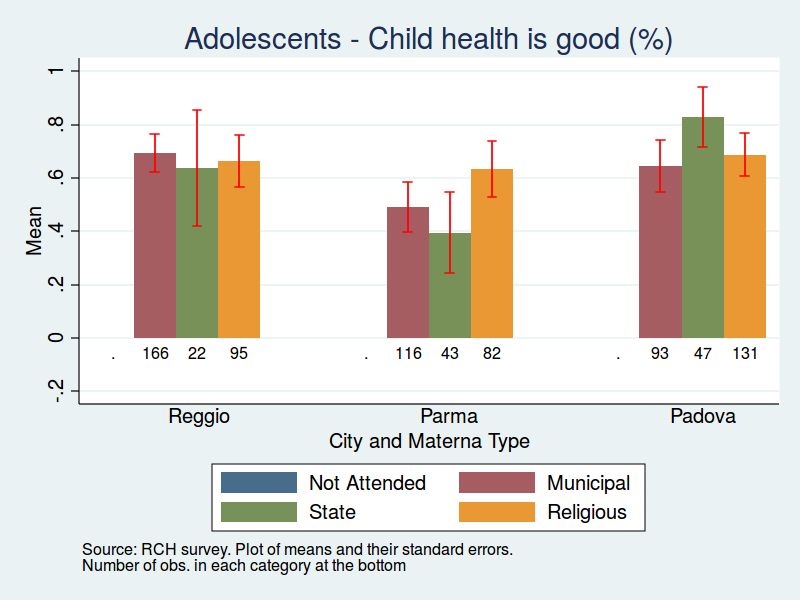
\includegraphics[scale=0.40]{../Output/childHealthPerc_Ado.png}
\end{frame}

%\begin{frame}
%\center
%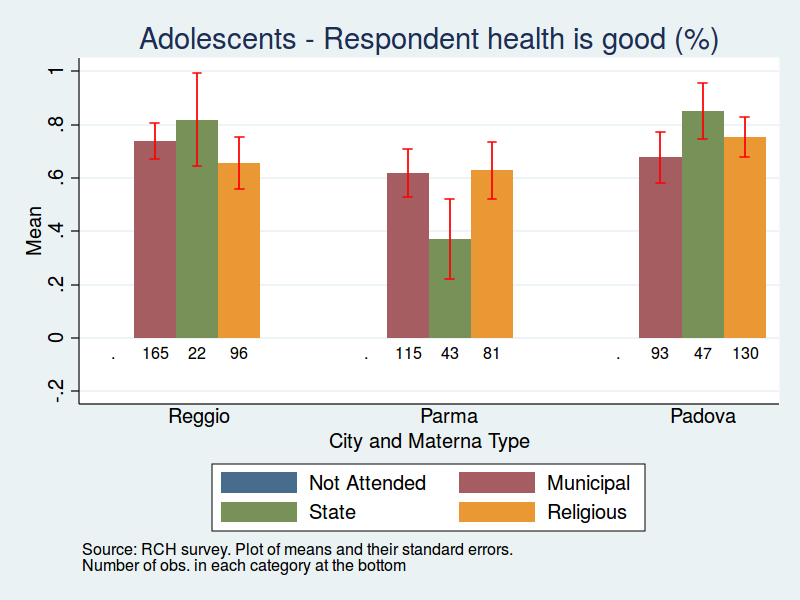
\includegraphics[scale=0.40]{../Output/HealthPerc_Ado.png}
%\end{frame}

\begin{frame}
\center
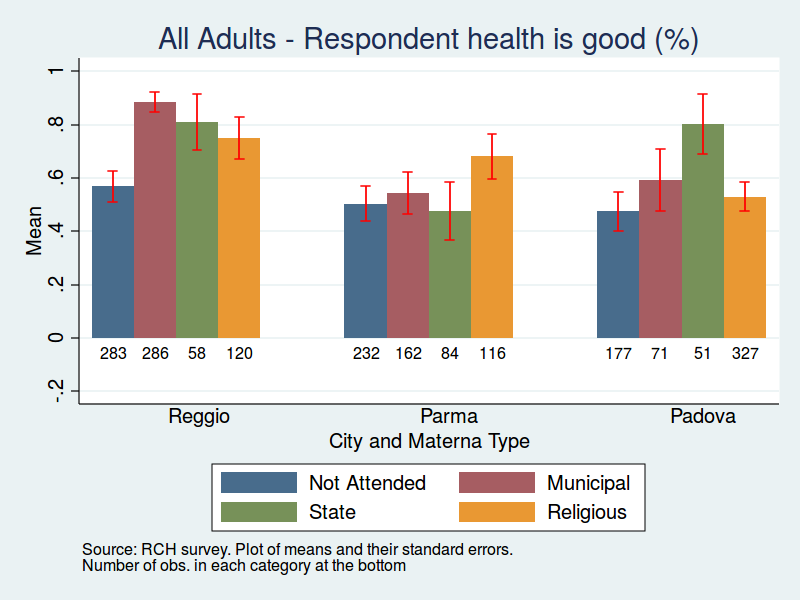
\includegraphics[scale=0.40]{../Output/HealthPerc_AllAdults.png}
\end{frame}

%%%%%%%%%%%% Attitudes Migrants %%%%%%%%%%%%%%%%%%%
\begin{frame}
\begin{itemize}
	\centering
	\item[4.] Negative attitudes towards migrants
	\begin{itemize}
		\centering
		\item Responded `very' or `quite' to the question ``Are you bothered by the immigration into the city?'' (5-point likert scale)
	\end{itemize}
\end{itemize}
\end{frame}

\begin{frame}
\center
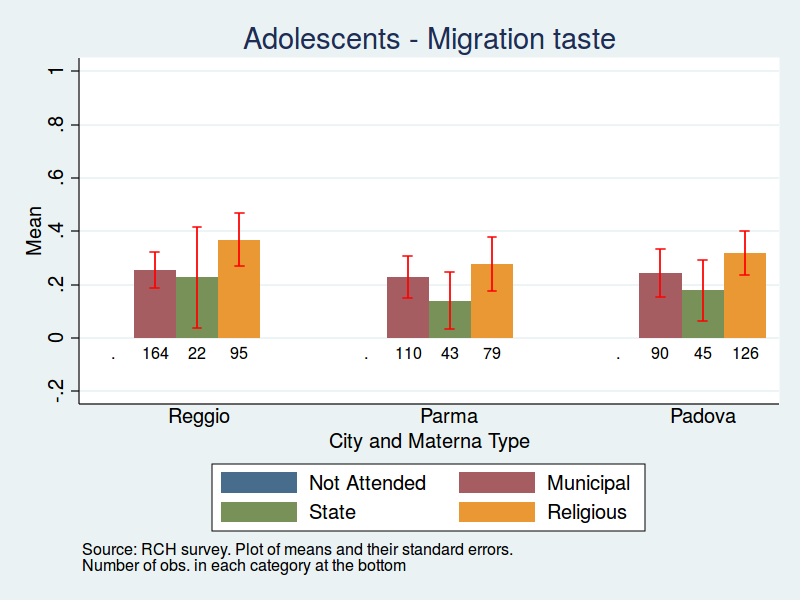
\includegraphics[scale=0.40]{../Output/MigrTaste_cat_Ado.png}
\end{frame}

\begin{frame}
\center
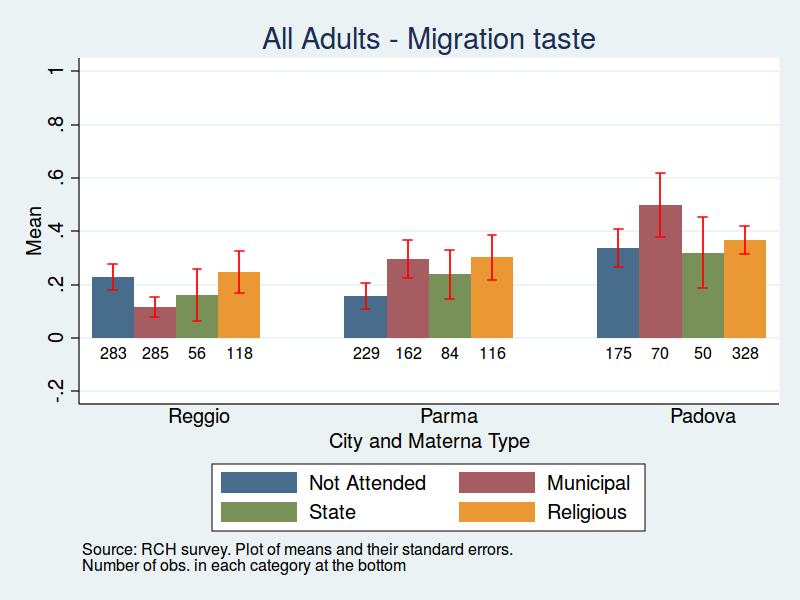
\includegraphics[scale=0.40]{../Output/MigrTaste_cat_AllAdults.png}
\end{frame}


%%%%%%%%%%
\section{Analysis: Conditional Correlations}
\begin{frame}\frametitle{Regression}
We now present the result of simple regressions that control incrementally for background variables that are determined before the choice of sending the children to child-care

\vspace{2ex}

\textbf{Separately} for each city, cohort, and age group we run the following:
\[ 
y = \alpha + \sum_{s} \delta_{s} D_{s} + \beta_{X}X + \varepsilon
\]

Where:
\begin{itemize}
%	\begin{small}
	\item $D_{s}$ are dummies for school type: municipal, state, private, not-attended
	\item The reference category is religious school
	\item The age groups are:
	\begin{itemize}
		\item age 0-3: choice of infant-toddler center 
		\item age 3-6: choice of preschool
		\item NOTE: there are no state infant-toddler centers, and virtually every child and adolescent attended some form of preschool
	\end{itemize}
%	\end{small}
\end{itemize}
\end{frame}

%%%%%%%%%%
\begin{frame}\frametitle{Controls Considered}
	\begin{itemize}
		\item Gender, age at interview, age$^2$
		\item Interviewer f.e., interview mode (computer or paper)
		\item dummies for parental education
		\item dummies for parents born in the region (province)
		\item dummies for family owns home, family income brackets
		\item dummies for low birthweight, born premature	
	\end{itemize}
\vspace{3ex}
\footnotesize See results in the appendix for incremental inclusion of controls.
\end{frame}

%%%%%%%%%%
\begin{frame}\frametitle{Output}
\begin{itemize}
	\item The following graphs report the estimated $\delta_{s}$ coefficients 
	\item The same graph combines results from 3 different regressions, one for every city
	\vspace{2ex}
	\item The $\delta_{s}$ coefficients represent differences in outcomes between school types, conditional on Xs
%	\item The purpose is to understand:
%	\begin{itemize}
%		\item how much these differences change as controls are included
%		\item which ones could be relevant control groups
%	\end{itemize}
\end{itemize}
\end{frame}

%%%%%%%%%%

\subsection{Strengths \& Difficulties}
%%%%%%%%%%%% SDQ %%%%%%%%%%%%%%%%%%%
\begin{frame}
\begin{itemize}
	\centering
	\item[1.] Strength and Difficulties Questionnaire
	\vspace{3ex}
	\begin{itemize}
		\item Reggio Children (RCH) associated with lower SDQ (better outcome)
		\begin{itemize}
			\item both for adolescents and children (once controlling for parental charact.)
			\item both for 0-3 and 3-6
		\end{itemize}
		\item Sometimes RCH not sig. different from not attended infant-toddler center, or state preschool (for adolescents)
		\vspace{2ex}
		\item Results in Parma are similar to Reggio, while in Padova religious schools seem to have lowest SDQ score (better outcome)
	\end{itemize}
\end{itemize}
\end{frame}
%-----------------------Child-----------------------%
%%%%%%%%%%% Asilo
\begin{frame}\frametitle{Child SDQ Score, age 0-3}
\center
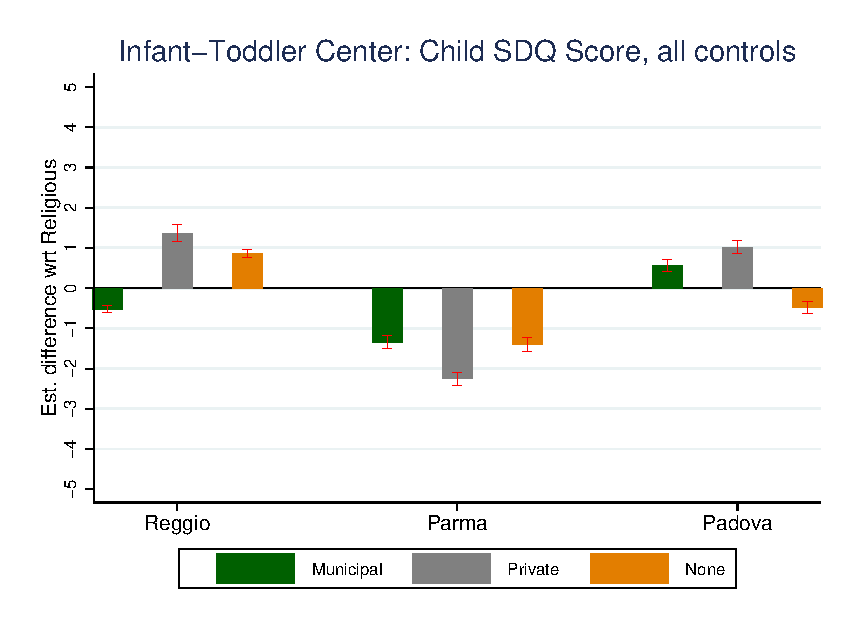
\includegraphics[scale=0.7]{../Output/graphs/CS_Asilo_Child_all.eps}
\end{frame}


%%%%%%%%%%% Materna
\begin{frame}\frametitle{Child SDQ Score,age 3-6}
\center
\includegraphics[scale=0.7]{../Output/graphs/CS_Materna_Child_all.eps}
\end{frame}

%-----------------------Adolescent%-----------------------%
%%%%%%%%%%% Asilo
\begin{frame}\frametitle{Adolescent SDQ Score, age 0-3}
\center
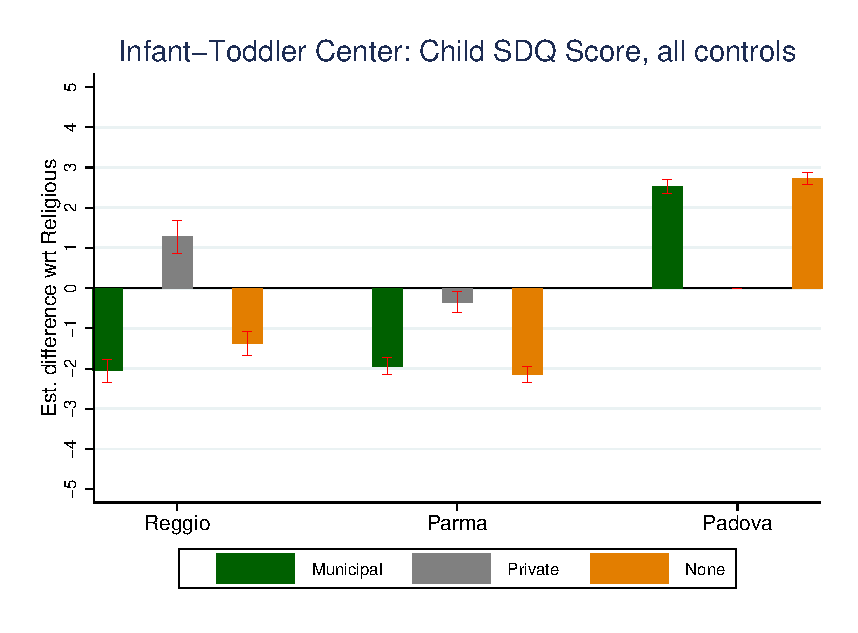
\includegraphics[scale=0.7]{../Output/graphs/CS_Asilo_Adol_all.eps}
\end{frame}

%%%%%%%%%%% Materna
\begin{frame}\frametitle{Adolescent SDQ Score,age 3-6}
\center
\includegraphics[scale=0.7]{../Output/graphs/CS_Materna_Adol_all.eps}
\end{frame}


\subsection{Depression}
%%%%%%%%%%%% Depression %%%%%%%%%%%%%%%%%%%
\begin{frame}
\begin{itemize}
	\centering
	\item[2.] Depression Score
	\vspace{3ex}
	\begin{itemize}
		\item No clear association with Reggio Children participation
		\begin{itemize}
			\item In both adolescents and adults, RCH is comparable to state, private, or no-school
			\item For adolescents, RCH seems better than religious, but not for adults
		\end{itemize}
		\vspace{2ex}
		\item Padova not-attended is a clear outlier (but with very few obs.)
		\item A lot of variability in both Parma and Padova
	\end{itemize}
\end{itemize}
\end{frame}

%-----------------------Adolescent%-----------------------%
%%%%%%%%%%% Asilo
\begin{frame}\frametitle{Adolescent Depression Score, age 0-3}
\center
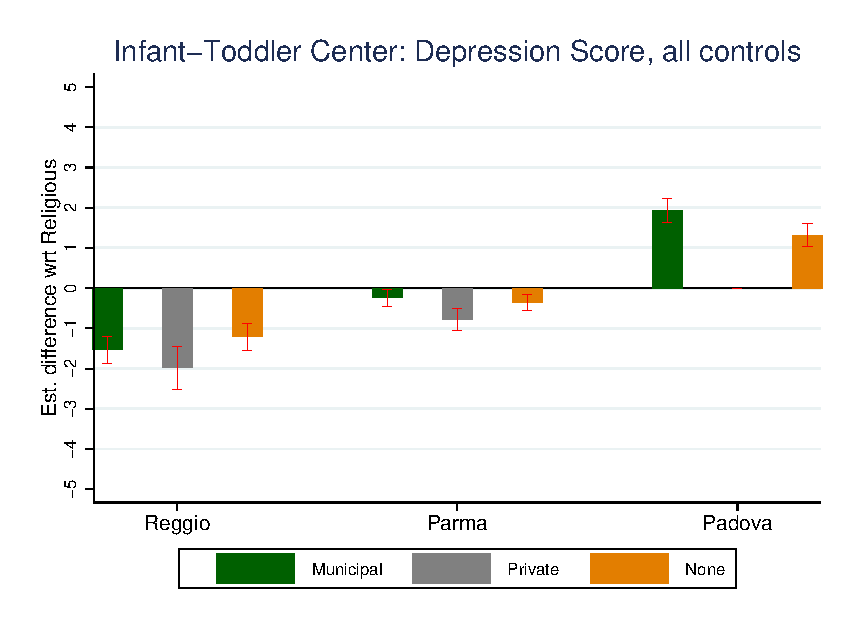
\includegraphics[scale=0.7]{../Output/graphs/D_Asilo_Adol_all.eps}
\end{frame}


%%%%%%%%%%% Materna
\begin{frame}\frametitle{Adolescent Depression Score,age 3-6}
\center
\includegraphics[scale=0.7]{../Output/graphs/D_Materna_Adol_all.eps}
\end{frame}

%-----------------------Adult%-----------------------%
%%%%%%%%%%% Asilo
\begin{frame}\frametitle{Adult Depression Score, age 0-3}
\center
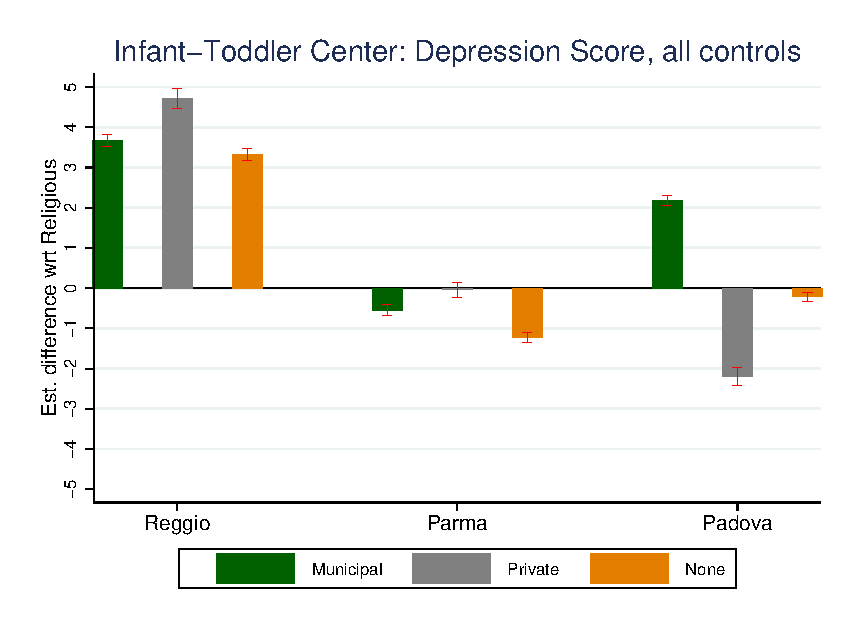
\includegraphics[scale=0.7]{../Output/graphs/D_Asilo_Adult_all.eps}
\end{frame}


%%%%%%%%%%% Materna
\begin{frame}\frametitle{Adult Depression Score,age 3-6}
\center
\includegraphics[scale=0.7]{../Output/graphs/D_Materna_Adult_all.eps}
\end{frame}


%%%%%%%%%%

\subsection{Health}
%%%%%%%%%%%% Health %%%%%%%%%%%%%%%%%%%
\begin{frame}
\begin{itemize}
	\centering
	\item[3.] Self-reported health
	\vspace{3ex}
	\begin{itemize}
		\item Very small differences across school types, especially for children and adolescents
		\begin{itemize}
			\item Note: children and adolescent attending Reggio Children have lower birthweight (negative selection)
			\item Adults attending a religious infant-toddler center are the only showing significant better health
		\end{itemize}
		\vspace{2ex}
		\item A lot of variability in both Parma and Padova
	\end{itemize}
\end{itemize}
\end{frame}

%-----------------------Child-----------------------%
%%%%%%%%%%% Asilo
\begin{frame}\frametitle{Child Health, age 0-3}
\center
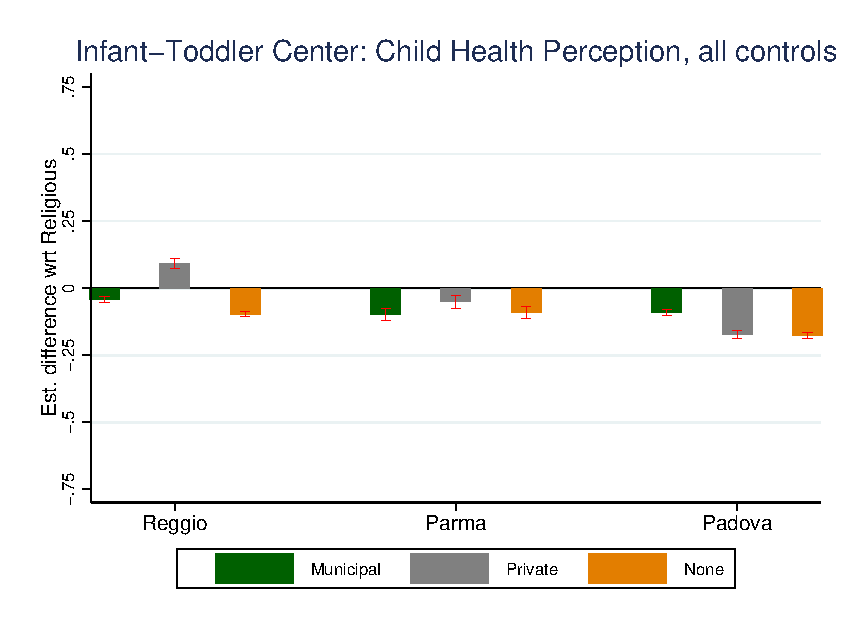
\includegraphics[scale=0.7]{../Output/graphs/CH_Asilo_Child_all.eps}
\end{frame}


%%%%%%%%%%% Materna
\begin{frame}\frametitle{Child Health,age 3-6}
\center
\includegraphics[scale=0.7]{../Output/graphs/CH_Materna_Child_all.eps}
\end{frame}

%-----------------------Adolescent%-----------------------%
%%%%%%%%%%% Asilo
\begin{frame}\frametitle{Adolescent Health, age 0-3}
\center
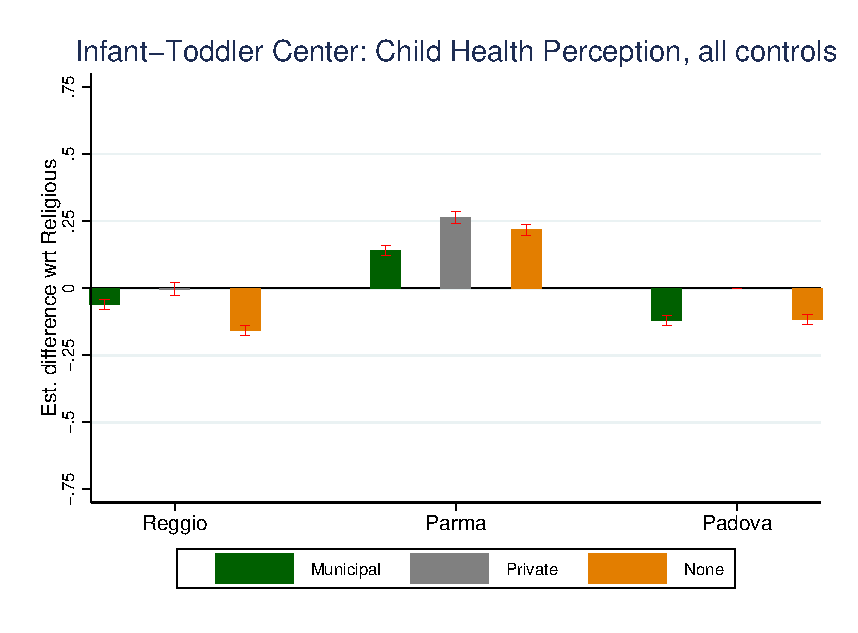
\includegraphics[scale=0.7]{../Output/graphs/CH_Asilo_Adol_all.eps}
\end{frame}


%%%%%%%%%%% Materna
\begin{frame}\frametitle{Adolescent Health,age 3-6}
\center
\includegraphics[scale=0.7]{../Output/graphs/CH_Materna_Adol_all.eps}
\end{frame}

%-----------------------Adult%-----------------------%
%%%%%%%%%%% Asilo
\begin{frame}\frametitle{Adult Health, age 0-3}
\center
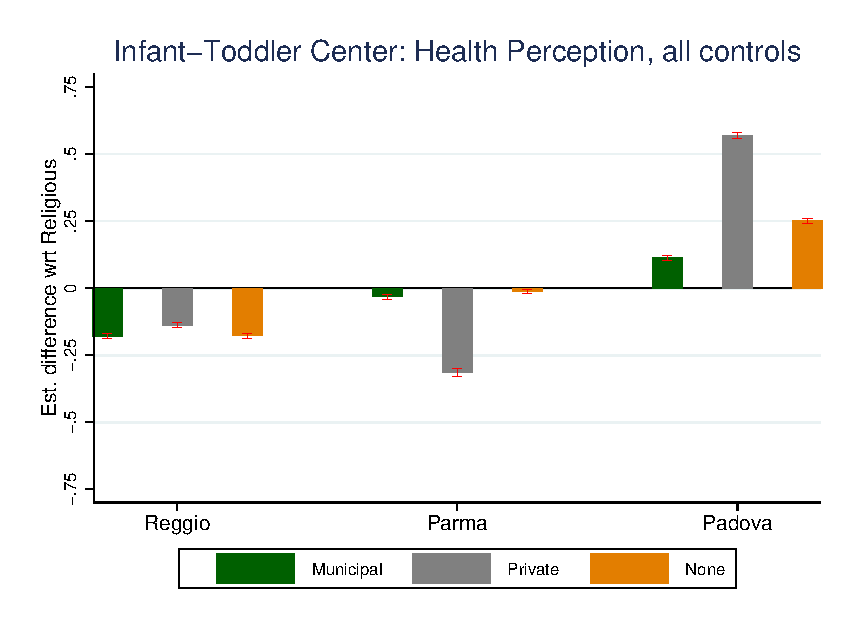
\includegraphics[scale=0.7]{../Output/graphs/H_Asilo_Adult_all.eps}
\end{frame}


%%%%%%%%%%% Materna
\begin{frame}\frametitle{Adult Health,age 3-6}
\center
\includegraphics[scale=0.7]{../Output/graphs/H_Materna_Adult_all.eps}
\end{frame}

\subsection{Attitudes Towards Migration}
%%%%%%%%%%%% Attitudes%%%%%%%%%%%%%%%%%%%
\begin{frame}
\begin{itemize}
	\centering
	\item[4.] Negative attitudes towards immigration into the city
	\vspace{3ex}
	\begin{itemize}
		\item Very small differences across school types, especially for adolescents
		\begin{itemize}
			\item Adolescents and adults attending religious schools seem to be less open to migrants
			\item Attendance to private schools is usually positively related to attitudes towards migrants
			\item Adolescents who attended Reggio Children infant-toddler centers seem to have negative attitudes, but the same is not true for those who attended Reggio Children preschools
		\end{itemize}
		\vspace{2ex}
		\item A lot of variability in both Parma and Padova
	\end{itemize}
\end{itemize}
\end{frame}

	%-----------------------Adolescent%-----------------------%
%%%%%%%%%%% Asilo
\begin{frame}\frametitle{Adolescent Attitudes towards migration, age 0-3}
\center
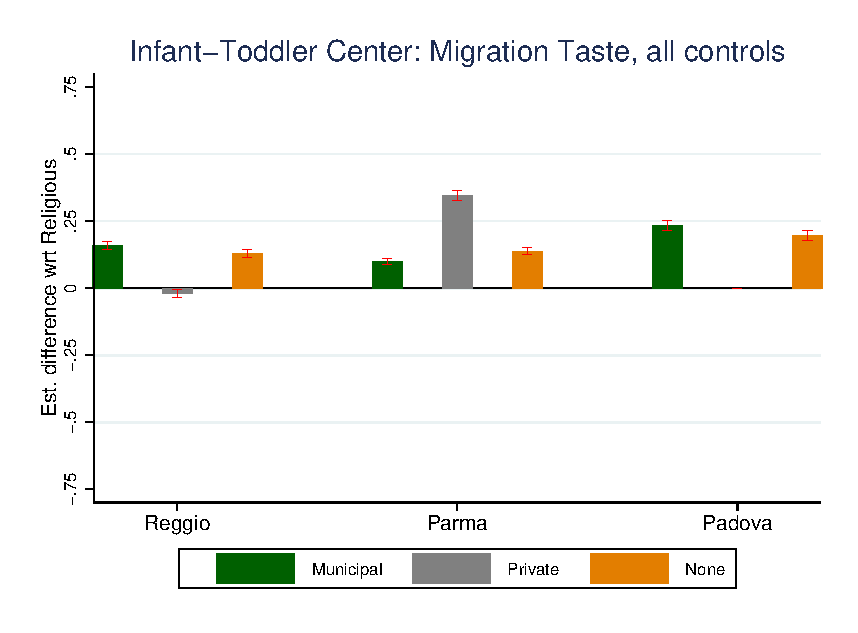
\includegraphics[scale=0.7]{../Output/graphs/M_Asilo_Adol_all.eps}
\end{frame}


%%%%%%%%%%% Materna
\begin{frame}\frametitle{Adolescent Attitudes towards migration,age 3-6}
\center
\includegraphics[scale=0.7]{../Output/graphs/M_Materna_Adol_all.eps}
\end{frame}

%-----------------------Adult%-----------------------%
%%%%%%%%%%% Asilo
\begin{frame}\frametitle{Adult Attitudes towards migration, age 0-3}
\center
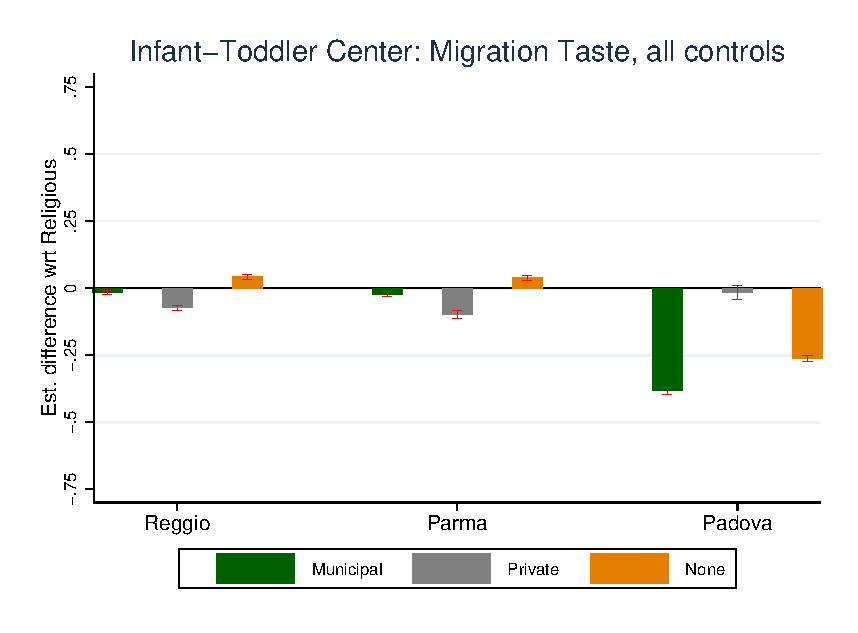
\includegraphics[scale=0.7]{../Output/graphs/M_Asilo_Adult_all.eps}
\end{frame}


%%%%%%%%%%% Materna
\begin{frame}\frametitle{Adult Attitudes towards migration,age 3-6}
\center
\includegraphics[scale=0.7]{../Output/graphs/M_Materna_Adult_all.eps}
\end{frame}

\section{Next Steps}
\begin{frame}\frametitle{Next Steps}
\begin{itemize}
	\item Understand selection into different type of schools
	\item Understand whether selection is similar across cities, and cohorts
	\item Identify relevant control groups
	\item Refine estimation strategy (propensity score, IV, etc.)
\end{itemize}
\end{frame}
%%%%%%%%%%
\section{Appendix}
\appendix

\begin{frame}
\center
\huge
Appendix: \\
Additional Tables
\end{frame}

\begin{frame}
\begin{tiny}
%\begin{table}[ht!]
\caption{\textbf{Completed Interviews and Response Rates}}
%\footnotesize
\label{tab:RespRate}
\begin{center}
\begin{tabular}{ l | c | c | c | c | c }
\hline\hline
\textbf{Cohort} & \multicolumn{2}{c}{\textbf{Reggio}} & \textbf{Parma} & \textbf{Padova} & \textbf{Total}\\
\hline
Children (yob 2006)       & Mun. & Rel.+St.+NoP. & Mun.+Rel.+St.+NoP. & Mun.+Rel.+St.+NoP.&\\[0.2em]
Italian (Cohort V)          & 160  & 151            & 291                & 278               & 880\\[0.2em]
\hline
\textit{Nov.2012-Aug.2013} & \multicolumn{2}{c|}{\textit{RR: 50.1\%}} & \textit{RR: 62.7\%} & \textit{RR: 50.1\%} & \textit{RR: 53.6\%}\\[0.2em]
\hline
Children (yob 2006)       & Mun. & Rel.+St.+NoP. & Mun.+Rel.+St.+NoP. & Mun.+Rel.+St.+NoP.&\\[0.2em]
Immigrant (Cohort V)        & 70   & 40             & 58                 & 113               & 281\\[0.2em]
\hline
\textit{Nov.2012-Aug.2013} & \multicolumn{2}{c|}{\textit{RR: 53.1\%}} & \textit{RR: 49.2\%} & \textit{RR: 63.1\%} & \textit{RR: 55.8\%}\\[0.2em]
\hline
Adolescents (yob 1994)    & Mun. & Rel.+St.+NoP. & Mun.+Rel.+St.+NoP. & Mun.+Rel.+St.+NoP.&\\[0.2em]
(Cohort IV)                 & 156  & 144            & 254                & 282               & 836\\[0.2em]
\hline
\textit{Nov.2012-Jul.2013} & \multicolumn{2}{c|}{\textit{RR: 57.1\%}} & \textit{RR: 58.5\%} & \textit{RR: 55.5\%} & \textit{RR: 57.0\%}\\[0.2em]
\hline
Adults (yob 1980-81)       & Mun. & Rel.+St.+NoP. & Mun.+Rel.+St.+NoP. & Mun.+Rel.+St.+NoP.&\\[0.2em]
(Cohort III)                 & 143  & 137            & 251                & 251               & 782\\[0.2em]
\hline
\textit{May 2013-Nov.2013} & \multicolumn{2}{c|}{\textit{RR: 58.3\%}} & \textit{RR: 58.2\%} & \textit{RR: 57.4\%} & \textit{RR: 58.0\%}\\[0.2em]
\hline
Adults (yob 1969-70)        & Mun. & Rel.+St.+NoP. & Mun.+Rel.+St.+NoP. & Mun.+Rel.+St.+NoP.&\\[0.2em]
(Cohort II)                   & 125  & 160            & 254                & 252               & 791\\[0.2em]
\hline
\textit{May 2013-Nov.2013} & \multicolumn{2}{c|}{\textit{RR: 59.3\%}} & \textit{RR: 56.3\%} & \textit{RR: 57.5\%} & \textit{RR: 57.7\%}\\[0.2em]
\hline
Adults (yob 1954-59)     & \multicolumn{2}{c|}{Mun.+Rel.+St.+NoP.} & Mun.+Rel.+St.+NoP. & Mun.+Rel.+St.+NoP.&\\[0.2em]
(Cohort I)                 & \multicolumn{2}{c|}{200} & 103 & 146 & 449\\[0.2em]
\hline
\textit{May 2013-Oct.2013} & \multicolumn{2}{c|}{\textit{RR: 52.2\%}} & \textit{RR: 63.6\%} & \textit{RR: 62.7\%} & \textit{RR: 57.7\%}\\[0.2em]
\hline 
\textbf{Total Interviews} & \multicolumn{2}{c|}{\textbf{1,486}} & \textbf{1,211} & \textbf{1,322} & \textbf{4,019} \\[0.2em]
\textit{Total Response Rates}       & \multicolumn{2}{c|}{\textit{55.1\%}} & \textit{58.8\%} & \textit{56.2\%} & \textit{56.5\%} \\
\hline
\end{tabular}
\end{center}
%\footnotesize
\tiny{{\bfseries Notes:} Mun.=Municipal Preschool; Rel.=Religious Preschool; St.=State Preschool; NoP.=No Preschool attended. yob=year of birth. For each cohort, the third line in the first column reports the interview periods. RR=response rate. The response rates are calculated as the ratio of interviews to total valid contacts. Valid contacts are the sum of: completed interviews, sharp refusal, no person present, talked with a relative, left paper questionnaire but never returned, interview began but not completed.}
\end{table} 
\begin{table}[ht!]
\caption{\textbf{Completed Interviews and Response Rates}}
%\footnotesize
\label{tab:RespRate}
\begin{center}
\begin{tabular}{ l | c | c | c | c | c }
\hline\hline
\textbf{Cohort} & \multicolumn{2}{c}{\textbf{Reggio}} & \textbf{Parma} & \textbf{Padova} & \textbf{Total}\\
\hline
Children (yob 2006)       & Mun. & Rel.+St.+NoP. & Mun.+Rel.+St.+NoP. & Mun.+Rel.+St.+NoP.&\\[0.2em]
Italian (Cohort V)          & 160  & 151            & 291                & 278               & 880\\[0.2em]
\hline
\textit{Nov.2012-Aug.2013} & \multicolumn{2}{c|}{\textit{RR: 50.1\%}} & \textit{RR: 62.7\%} & \textit{RR: 50.1\%} & \textit{RR: 53.6\%}\\[0.2em]
\hline
Children (yob 2006)       & Mun. & Rel.+St.+NoP. & Mun.+Rel.+St.+NoP. & Mun.+Rel.+St.+NoP.&\\[0.2em]
Immigrant (Cohort V)        & 70   & 40             & 58                 & 113               & 281\\[0.2em]
\hline
\textit{Nov.2012-Aug.2013} & \multicolumn{2}{c|}{\textit{RR: 53.1\%}} & \textit{RR: 49.2\%} & \textit{RR: 63.1\%} & \textit{RR: 55.8\%}\\[0.2em]
\hline
Adolescents (yob 1994)    & Mun. & Rel.+St.+NoP. & Mun.+Rel.+St.+NoP. & Mun.+Rel.+St.+NoP.&\\[0.2em]
(Cohort IV)                 & 156  & 144            & 254                & 282               & 836\\[0.2em]
\hline
\textit{Nov.2012-Jul.2013} & \multicolumn{2}{c|}{\textit{RR: 57.1\%}} & \textit{RR: 58.5\%} & \textit{RR: 55.5\%} & \textit{RR: 57.0\%}\\[0.2em]
\hline
Adults (yob 1980-81)       & Mun. & Rel.+St.+NoP. & Mun.+Rel.+St.+NoP. & Mun.+Rel.+St.+NoP.&\\[0.2em]
(Cohort III)                 & 143  & 137            & 251                & 251               & 782\\[0.2em]
\hline
\textit{May 2013-Nov.2013} & \multicolumn{2}{c|}{\textit{RR: 58.3\%}} & \textit{RR: 58.2\%} & \textit{RR: 57.4\%} & \textit{RR: 58.0\%}\\[0.2em]
\hline
Adults (yob 1969-70)        & Mun. & Rel.+St.+NoP. & Mun.+Rel.+St.+NoP. & Mun.+Rel.+St.+NoP.&\\[0.2em]
(Cohort II)                   & 125  & 160            & 254                & 252               & 791\\[0.2em]
\hline
\textit{May 2013-Nov.2013} & \multicolumn{2}{c|}{\textit{RR: 59.3\%}} & \textit{RR: 56.3\%} & \textit{RR: 57.5\%} & \textit{RR: 57.7\%}\\[0.2em]
\hline
Adults (yob 1954-59)     & \multicolumn{2}{c|}{Mun.+Rel.+St.+NoP.} & Mun.+Rel.+St.+NoP. & Mun.+Rel.+St.+NoP.&\\[0.2em]
(Cohort I)                 & \multicolumn{2}{c|}{200} & 103 & 146 & 449\\[0.2em]
\hline
\textit{May 2013-Oct.2013} & \multicolumn{2}{c|}{\textit{RR: 52.2\%}} & \textit{RR: 63.6\%} & \textit{RR: 62.7\%} & \textit{RR: 57.7\%}\\[0.2em]
\hline 
\textbf{Total Interviews} & \multicolumn{2}{c|}{\textbf{1,486}} & \textbf{1,211} & \textbf{1,322} & \textbf{4,019} \\[0.2em]
\textit{Total Response Rates}       & \multicolumn{2}{c|}{\textit{55.1\%}} & \textit{58.8\%} & \textit{56.2\%} & \textit{56.5\%} \\
\hline
\end{tabular}
\end{center}
%\footnotesize
\tiny{{\bfseries Notes:} Mun.=Municipal Preschool; Rel.=Religious Preschool; St.=State Preschool; NoP.=No Preschool attended. yob=year of birth. For each cohort, the third line in the first column reports the interview periods. RR=response rate. The response rates are calculated as the ratio of interviews to total valid contacts. Valid contacts are the sum of: completed interviews, sharp refusal, no person present, talked with a relative, left paper questionnaire but never returned, interview began but not completed.}
\end{table} 
\end{tiny}
\end{frame}

%%%%%%%%%%%%% Depression %%%%%%%%%%%%%%%%%%%
%\begin{frame}
%\begin{itemize}
%	\item[2.] Depression CES-D scale
%	\begin{itemize}
%		\item Raw score, ranging from 10 to 50
%	\end{itemize}
%\end{itemize}
%\end{frame}
%
%\begin{frame}
%\center
%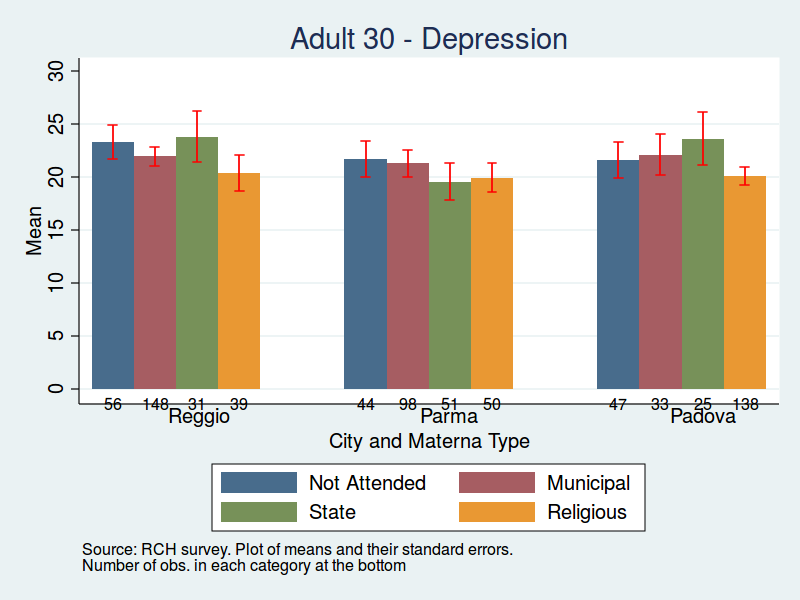
\includegraphics[scale=0.40]{../Output/Depression_score_Adult30.png}
%\end{frame}
%
%\begin{frame}
%\center
%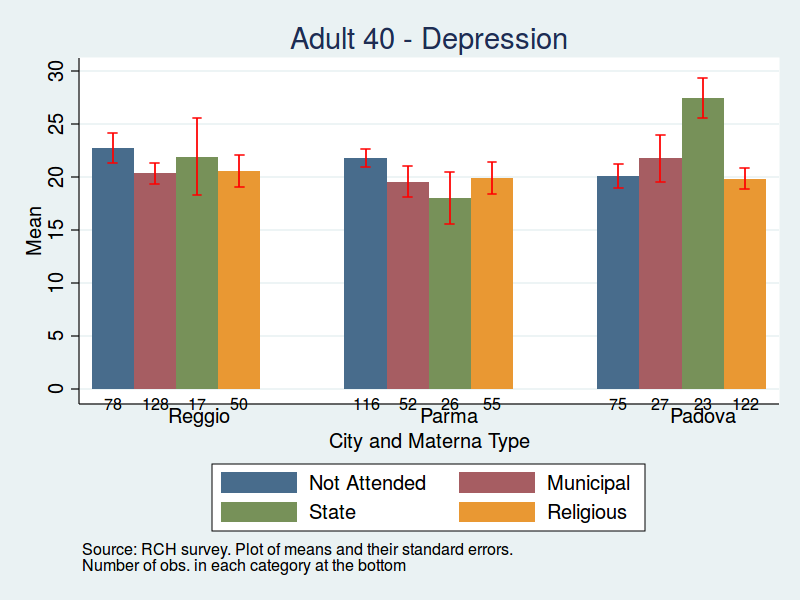
\includegraphics[scale=0.40]{../Output/Depression_score_Adult40.png}
%\end{frame}
%
%\begin{frame}
%\center
%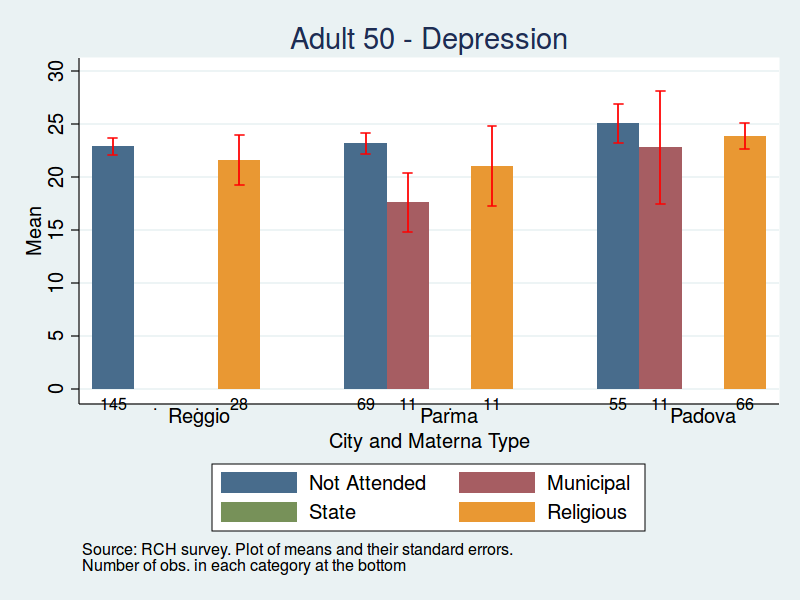
\includegraphics[scale=0.40]{../Output/Depression_score_Adult50.png}
%\end{frame}

%%%%%%%%%%
\begin{frame}\frametitle{Incrementally Add Controls}
We incrementally included all of the following set of controls. \\
The graphs below show the change in the coefficients as more controls are included.
	\begin{itemize}
		\item Set 1:
		\begin{itemize}
			\item none
		\end{itemize}
		\item Set 2: adding ...
		\begin{itemize}
			\item Gender, age at interview, age$^2$
			\item Interviewer f.e., interview mode (computer or paper)
		\end{itemize}
		\item Set 3: adding ...
		\begin{itemize}
			\item dummies for parental education
			\item dummies for parents born in the region (province)
			\item dummies for family owns home, family income brackets
		\end{itemize}
		\item Set 4: adding ...
		\begin{itemize}
			\item dummies for low birthweight, born premature	
		\end{itemize}
	\end{itemize}
\end{frame}
  
\subsection{Strengths \& Difficulties}
%%%%%%%%%%%% SDQ %%%%%%%%%%%%%%%%%%%
\begin{frame}
\begin{itemize}
	\centering
	\item[1.] Strength and Difficulties Questionnaire
\end{itemize}
\end{frame}
%-----------------------Child-----------------------%
%%%%%%%%%%% Asilo
\begin{frame}\frametitle{Child SDQ Score, age 0-3}
\center
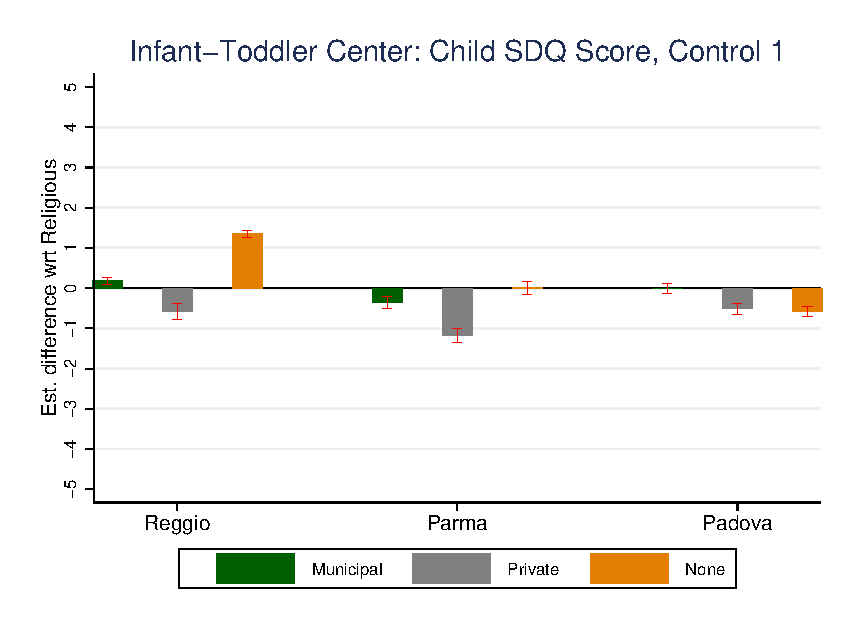
\includegraphics[scale=0.7]{../Output/graphs/CS_Asilo_Child_main.eps}
\end{frame}

\begin{frame}\frametitle{Child SDQ Score, age 0-3}
\center
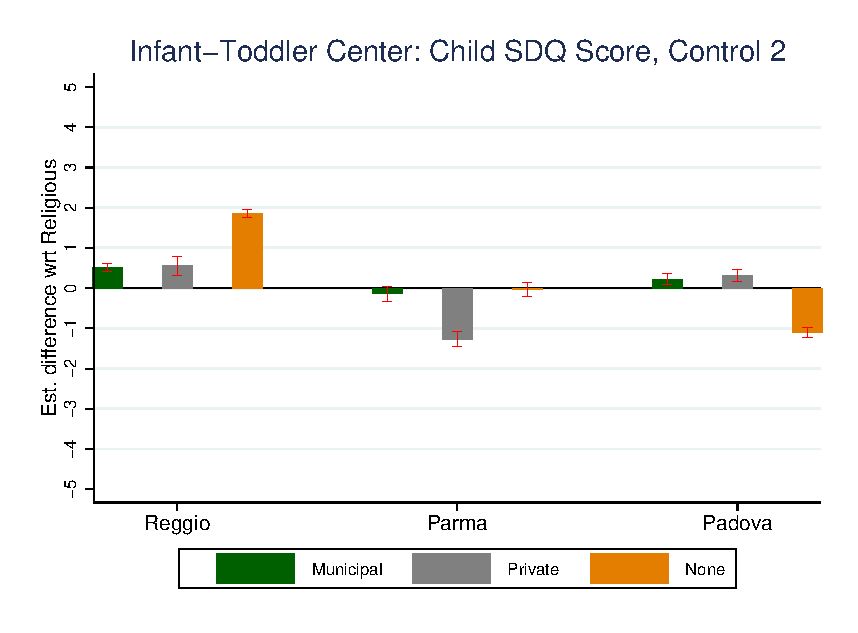
\includegraphics[scale=0.7]{../Output/graphs/CS_Asilo_Child_inter.eps}
\end{frame}

\begin{frame}\frametitle{Child SDQ Score, age 0-3}
\center
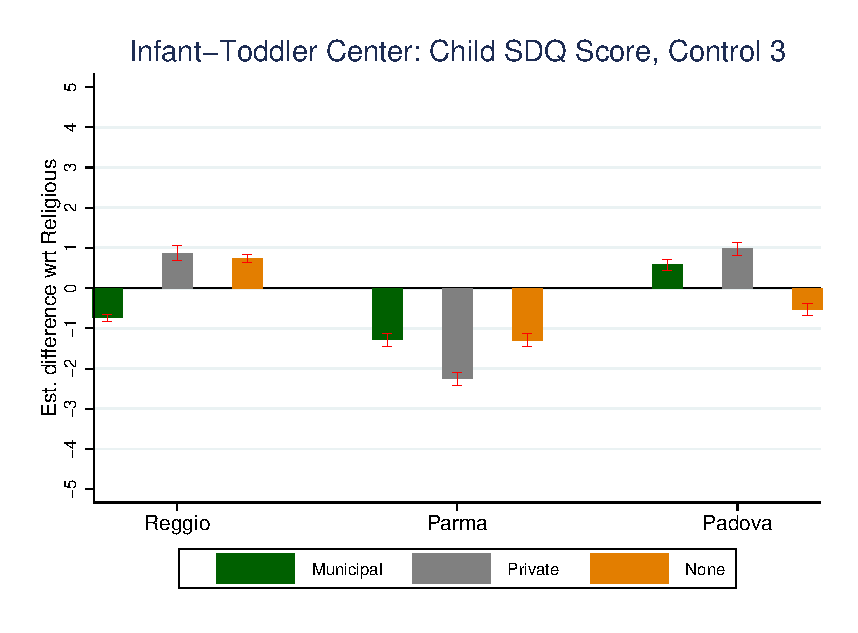
\includegraphics[scale=0.7]{../Output/graphs/CS_Asilo_Child_right.eps}
\end{frame}

\begin{frame}\frametitle{Child SDQ Score, age 0-3}
\center
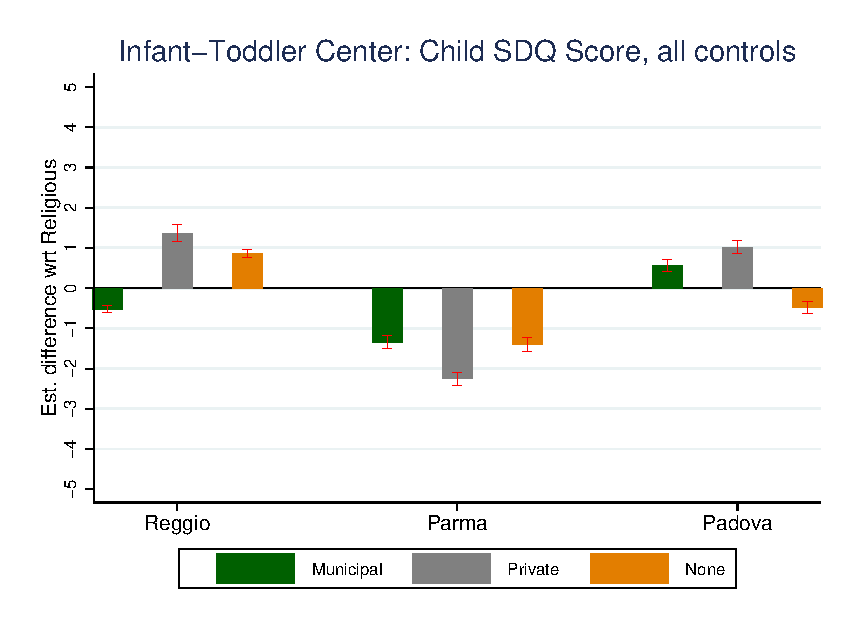
\includegraphics[scale=0.7]{../Output/graphs/CS_Asilo_Child_all.eps}
\end{frame}


%%%%%%%%%%% Materna
\begin{frame}\frametitle{Child SDQ Score, age 3-6}
\center
\includegraphics[scale=0.7]{../Output/graphs/CS_Materna_Child_main.eps}
\end{frame}

\begin{frame}\frametitle{Child SDQ Score, age 3-6}
\center
\includegraphics[scale=0.7]{../Output/graphs/CS_Materna_Child_inter.eps}
\end{frame}

\begin{frame}\frametitle{Child SDQ Score,age 3-6}
\center
\includegraphics[scale=0.7]{../Output/graphs/CS_Materna_Child_right.eps}
\end{frame}

\begin{frame}\frametitle{Child SDQ Score,age 3-6}
\center
\includegraphics[scale=0.7]{../Output/graphs/CS_Materna_Child_all.eps}
\end{frame}

%-----------------------Adolescent%-----------------------%
%%%%%%%%%%% Asilo
\begin{frame}\frametitle{Adolescent SDQ Score, age 0-3}
\center
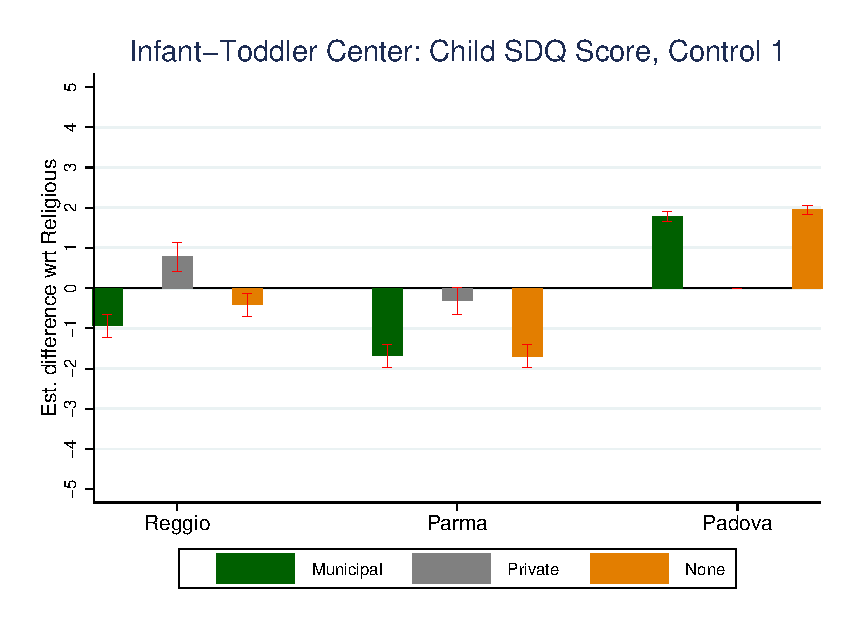
\includegraphics[scale=0.7]{../Output/graphs/CS_Asilo_Adol_main.eps}
\end{frame}

\begin{frame}\frametitle{Adolescent SDQ Score, age 0-3}
\center
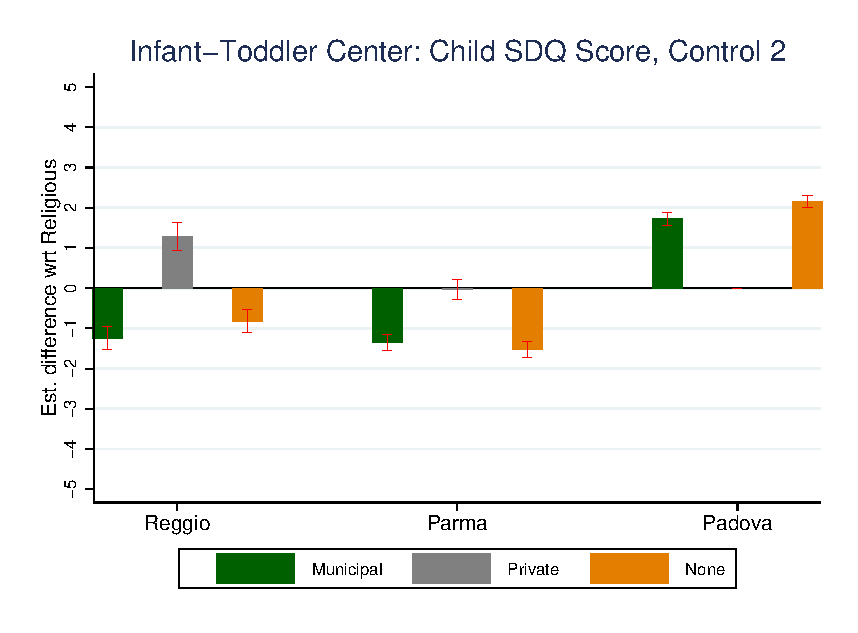
\includegraphics[scale=0.7]{../Output/graphs/CS_Asilo_Adol_inter.eps}
\end{frame}

\begin{frame}\frametitle{Adolescent SDQ Score, age 0-3}
\center
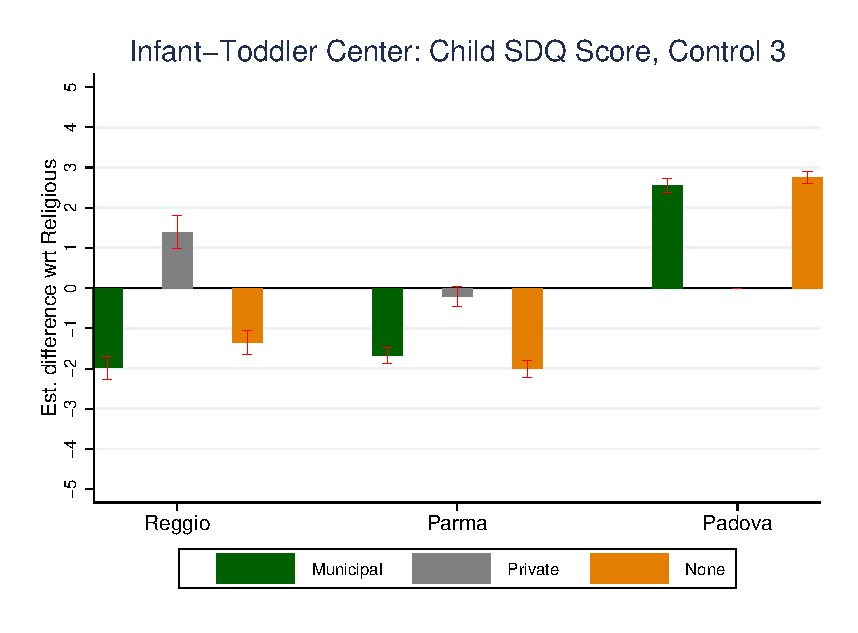
\includegraphics[scale=0.7]{../Output/graphs/CS_Asilo_Adol_right.eps}
\end{frame}

\begin{frame}\frametitle{Adolescent SDQ Score, age 0-3}
\center
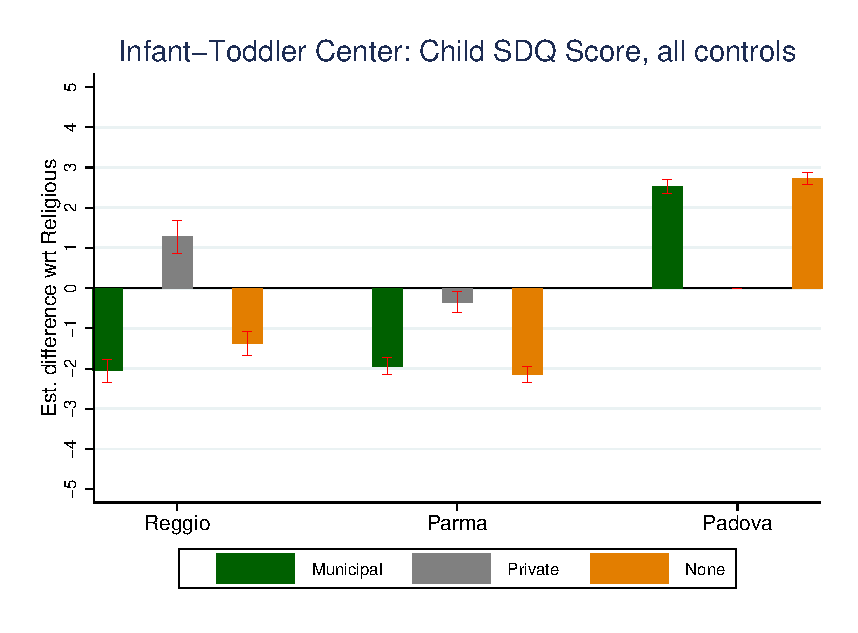
\includegraphics[scale=0.7]{../Output/graphs/CS_Asilo_Adol_all.eps}
\end{frame}


%%%%%%%%%%% Materna
\begin{frame}\frametitle{Adolescent SDQ Score, age 3-6}
\center
\includegraphics[scale=0.7]{../Output/graphs/CS_Materna_Adol_main.eps}
\end{frame}

\begin{frame}\frametitle{Adolescent SDQ Score, age 3-6}
\center
\includegraphics[scale=0.7]{../Output/graphs/CS_Materna_Adol_inter.eps}
\end{frame}

\begin{frame}\frametitle{Adolescent SDQ Score,age 3-6}
\center
\includegraphics[scale=0.7]{../Output/graphs/CS_Materna_Adol_right.eps}
\end{frame}

\begin{frame}\frametitle{Adolescent SDQ Score,age 3-6}
\center
\includegraphics[scale=0.7]{../Output/graphs/CS_Materna_Adol_all.eps}
\end{frame}


\subsection{Depression}
%%%%%%%%%%%% Depression %%%%%%%%%%%%%%%%%%%
\begin{frame}
\begin{itemize}
	\centering
	\item[2.] Depression Score
\end{itemize}
\end{frame}

%-----------------------Adolescent%-----------------------%
%%%%%%%%%%% Asilo
\begin{frame}\frametitle{Adolescent Depression Score, age 0-3}
\center
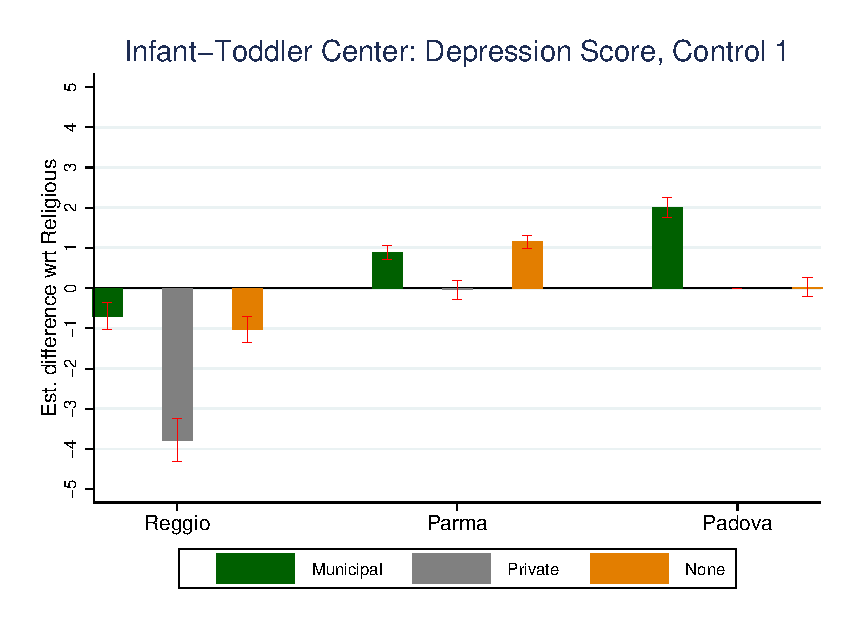
\includegraphics[scale=0.7]{../Output/graphs/D_Asilo_Adol_main.eps}
\end{frame}

\begin{frame}\frametitle{Adolescent Depression Score, age 0-3}
\center
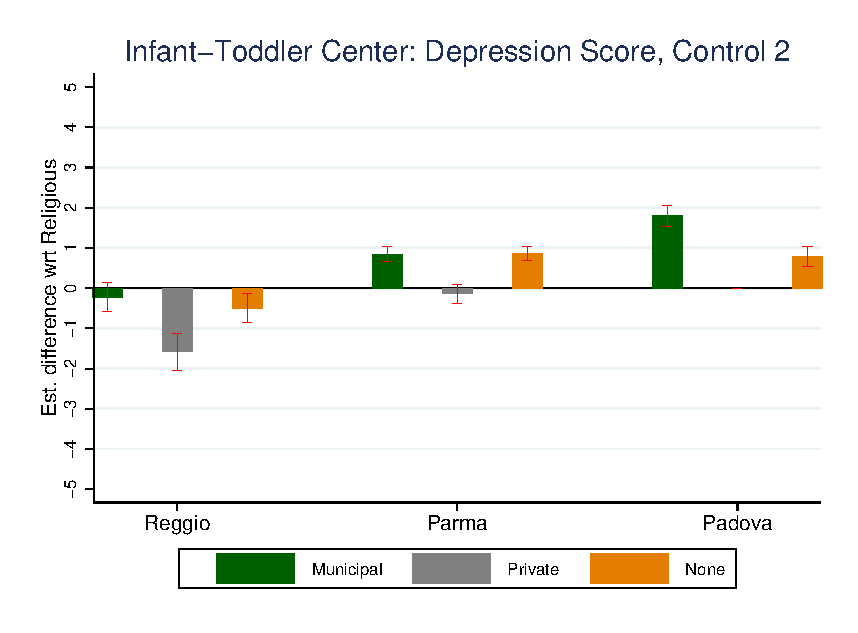
\includegraphics[scale=0.7]{../Output/graphs/D_Asilo_Adol_inter.eps}
\end{frame}

\begin{frame}\frametitle{Adolescent Depression Score, age 0-3}
\center
\includegraphics[scale=0.7]{../Output/graphs/D_Asilo_Adol_right.eps}
\end{frame}

\begin{frame}\frametitle{Adolescent Depression Score, age 0-3}
\center
\includegraphics[scale=0.7]{../Output/graphs/D_Asilo_Adol_all.eps}
\end{frame}


%%%%%%%%%%% Materna
\begin{frame}\frametitle{Adolescent Depression Score, age 3-6}
\center
\includegraphics[scale=0.7]{../Output/graphs/D_Materna_Adol_main.eps}
\end{frame}

\begin{frame}\frametitle{Adolescent Depression Score, age 3-6}
\center
\includegraphics[scale=0.7]{../Output/graphs/D_Materna_Adol_inter.eps}
\end{frame}

\begin{frame}\frametitle{Adolescent Depression Score,age 3-6}
\center
\includegraphics[scale=0.7]{../Output/graphs/D_Materna_Adol_right.eps}
\end{frame}

\begin{frame}\frametitle{Adolescent Depression Score,age 3-6}
\center
\includegraphics[scale=0.7]{../Output/graphs/D_Materna_Adol_all.eps}
\end{frame}

%-----------------------Adult%-----------------------%
%%%%%%%%%%% Asilo
\begin{frame}\frametitle{Adult Depression Score, age 0-3}
\center
\includegraphics[scale=0.7]{../Output/graphs/D_Asilo_Adult_main.eps}
\end{frame}

\begin{frame}\frametitle{Adult Depression Score, age 0-3}
\center
\includegraphics[scale=0.7]{../Output/graphs/D_Asilo_Adult_inter.eps}
\end{frame}

\begin{frame}\frametitle{Adult Depression Score, age 0-3}
\center
\includegraphics[scale=0.7]{../Output/graphs/D_Asilo_Adult_right.eps}
\end{frame}

\begin{frame}\frametitle{Adult Depression Score, age 0-3}
\center
\includegraphics[scale=0.7]{../Output/graphs/D_Asilo_Adult_all.eps}
\end{frame}


%%%%%%%%%%% Materna
\begin{frame}\frametitle{Adult Depression Score, age 3-6}
\center
\includegraphics[scale=0.7]{../Output/graphs/D_Materna_Adult_main.eps}
\end{frame}

\begin{frame}\frametitle{Adult Depression Score, age 3-6}
\center
\includegraphics[scale=0.7]{../Output/graphs/D_Materna_Adult_inter.eps}
\end{frame}

\begin{frame}\frametitle{Adult Depression Score,age 3-6}
\center
\includegraphics[scale=0.7]{../Output/graphs/D_Materna_Adult_right.eps}
\end{frame}

\begin{frame}\frametitle{Adult Depression Score,age 3-6}
\center
\includegraphics[scale=0.7]{../Output/graphs/D_Materna_Adult_all.eps}
\end{frame}


%%%%%%%%%%

\subsection{Health}
%%%%%%%%%%%% Health %%%%%%%%%%%%%%%%%%%
\begin{frame}
\begin{itemize}
	\centering
	\item[3.] Self-reported health
\end{itemize}
\end{frame}

%-----------------------Child-----------------------%
%%%%%%%%%%% Asilo
\begin{frame}\frametitle{Child Health, age 0-3}
\center
\includegraphics[scale=0.7]{../Output/graphs/CH_Asilo_Child_main.eps}
\end{frame}

\begin{frame}\frametitle{Child Health, age 0-3}
\center
\includegraphics[scale=0.7]{../Output/graphs/CH_Asilo_Child_inter.eps}
\end{frame}

\begin{frame}\frametitle{Child Health, age 0-3}
\center
\includegraphics[scale=0.7]{../Output/graphs/CH_Asilo_Child_right.eps}
\end{frame}

\begin{frame}\frametitle{Child Health, age 0-3}
\center
\includegraphics[scale=0.7]{../Output/graphs/CH_Asilo_Child_all.eps}
\end{frame}


%%%%%%%%%%% Materna
\begin{frame}\frametitle{Child Health, age 3-6}
\center
\includegraphics[scale=0.7]{../Output/graphs/CH_Materna_Child_main.eps}
\end{frame}

\begin{frame}\frametitle{Child Health, age 3-6}
\center
\includegraphics[scale=0.7]{../Output/graphs/CH_Materna_Child_inter.eps}
\end{frame}

\begin{frame}\frametitle{Child Health,age 3-6}
\center
\includegraphics[scale=0.7]{../Output/graphs/CH_Materna_Child_right.eps}
\end{frame}

\begin{frame}\frametitle{Child Health,age 3-6}
\center
\includegraphics[scale=0.7]{../Output/graphs/CH_Materna_Child_all.eps}
\end{frame}

%-----------------------Adolescent%-----------------------%
%%%%%%%%%%% Asilo
\begin{frame}\frametitle{Adolescent Health, age 0-3}
\center
\includegraphics[scale=0.7]{../Output/graphs/CH_Asilo_Adol_main.eps}
\end{frame}

\begin{frame}\frametitle{Adolescent Health, age 0-3}
\center
\includegraphics[scale=0.7]{../Output/graphs/CH_Asilo_Adol_inter.eps}
\end{frame}

\begin{frame}\frametitle{Adolescent Health, age 0-3}
\center
\includegraphics[scale=0.7]{../Output/graphs/CH_Asilo_Adol_right.eps}
\end{frame}

\begin{frame}\frametitle{Adolescent Health, age 0-3}
\center
\includegraphics[scale=0.7]{../Output/graphs/CH_Asilo_Adol_all.eps}
\end{frame}


%%%%%%%%%%% Materna
\begin{frame}\frametitle{Adolescent Health, age 3-6}
\center
\includegraphics[scale=0.7]{../Output/graphs/CH_Materna_Adol_main.eps}
\end{frame}

\begin{frame}\frametitle{Adolescent Health, age 3-6}
\center
\includegraphics[scale=0.7]{../Output/graphs/CH_Materna_Adol_inter.eps}
\end{frame}

\begin{frame}\frametitle{Adolescent Health,age 3-6}
\center
\includegraphics[scale=0.7]{../Output/graphs/CH_Materna_Adol_right.eps}
\end{frame}

\begin{frame}\frametitle{Adolescent Health,age 3-6}
\center
\includegraphics[scale=0.7]{../Output/graphs/CH_Materna_Adol_all.eps}
\end{frame}

%-----------------------Adult%-----------------------%
%%%%%%%%%%% Asilo
\begin{frame}\frametitle{Adult Health, age 0-3}
\center
\includegraphics[scale=0.7]{../Output/graphs/H_Asilo_Adult_main.eps}
\end{frame}

\begin{frame}\frametitle{Adult Health, age 0-3}
\center
\includegraphics[scale=0.7]{../Output/graphs/H_Asilo_Adult_inter.eps}
\end{frame}

\begin{frame}\frametitle{Adult Health, age 0-3}
\center
\includegraphics[scale=0.7]{../Output/graphs/H_Asilo_Adult_right.eps}
\end{frame}

\begin{frame}\frametitle{Adult Health, age 0-3}
\center
\includegraphics[scale=0.7]{../Output/graphs/H_Asilo_Adult_all.eps}
\end{frame}


%%%%%%%%%%% Materna
\begin{frame}\frametitle{Adult Health, age 3-6}
\center
\includegraphics[scale=0.7]{../Output/graphs/H_Materna_Adult_main.eps}
\end{frame}

\begin{frame}\frametitle{Adult Health, age 3-6}
\center
\includegraphics[scale=0.7]{../Output/graphs/H_Materna_Adult_inter.eps}
\end{frame}

\begin{frame}\frametitle{Adult Health,age 3-6}
\center
\includegraphics[scale=0.7]{../Output/graphs/H_Materna_Adult_right.eps}
\end{frame}

\begin{frame}\frametitle{Adult Health,age 3-6}
\center
\includegraphics[scale=0.7]{../Output/graphs/H_Materna_Adult_all.eps}
\end{frame}

\subsection{Attitudes Towards Migration}
%%%%%%%%%%%% Attitudes%%%%%%%%%%%%%%%%%%%
\begin{frame}
\begin{itemize}
	\centering
	\item[4.] Negative attitudes towards migrants
\end{itemize}
\end{frame}

	%-----------------------Adolescent%-----------------------%
%%%%%%%%%%% Asilo
\begin{frame}\frametitle{Adolescent Attitudes towards migration, age 0-3}
\center
\includegraphics[scale=0.7]{../Output/graphs/M_Asilo_Adol_main.eps}
\end{frame}

\begin{frame}\frametitle{Adolescent Attitudes towards migration, age 0-3}
\center
\includegraphics[scale=0.7]{../Output/graphs/M_Asilo_Adol_inter.eps}
\end{frame}

\begin{frame}\frametitle{Adolescent Attitudes towards migration, age 0-3}
\center
\includegraphics[scale=0.7]{../Output/graphs/M_Asilo_Adol_right.eps}
\end{frame}

\begin{frame}\frametitle{Adolescent Attitudes towards migration, age 0-3}
\center
\includegraphics[scale=0.7]{../Output/graphs/M_Asilo_Adol_all.eps}
\end{frame}


%%%%%%%%%%% Materna
\begin{frame}\frametitle{Adolescent Attitudes towards migration, age 3-6}
\center
\includegraphics[scale=0.7]{../Output/graphs/M_Materna_Adol_main.eps}
\end{frame}

\begin{frame}\frametitle{Adolescent Attitudes towards migration, age 3-6}
\center
\includegraphics[scale=0.7]{../Output/graphs/M_Materna_Adol_inter.eps}
\end{frame}

\begin{frame}\frametitle{Adolescent Attitudes towards migration,age 3-6}
\center
\includegraphics[scale=0.7]{../Output/graphs/M_Materna_Adol_right.eps}
\end{frame}

\begin{frame}\frametitle{Adolescent Attitudes towards migration,age 3-6}
\center
\includegraphics[scale=0.7]{../Output/graphs/M_Materna_Adol_all.eps}
\end{frame}

%-----------------------Adult%-----------------------%
%%%%%%%%%%% Asilo
\begin{frame}\frametitle{Adult Attitudes towards migration, age 0-3}
\center
\includegraphics[scale=0.7]{../Output/graphs/M_Asilo_Adult_main.eps}
\end{frame}

\begin{frame}\frametitle{Adult Attitudes towards migration, age 0-3}
\center
\includegraphics[scale=0.7]{../Output/graphs/M_Asilo_Adult_inter.eps}
\end{frame}

\begin{frame}\frametitle{Adult Attitudes towards migration, age 0-3}
\center
\includegraphics[scale=0.7]{../Output/graphs/M_Asilo_Adult_right.eps}
\end{frame}

\begin{frame}\frametitle{Adult Attitudes towards migration, age 0-3}
\center
\includegraphics[scale=0.7]{../Output/graphs/M_Asilo_Adult_all.eps}
\end{frame}


%%%%%%%%%%% Materna
\begin{frame}\frametitle{Adult Attitudes towards migration, age 3-6}
\center
\includegraphics[scale=0.7]{../Output/graphs/M_Materna_Adult_main.eps}
\end{frame}

\begin{frame}\frametitle{Adult Attitudes towards migration, age 3-6}
\center
\includegraphics[scale=0.7]{../Output/graphs/M_Materna_Adult_inter.eps}
\end{frame}

\begin{frame}\frametitle{Adult Attitudes towards migration,age 3-6}
\center
\includegraphics[scale=0.7]{../Output/graphs/M_Materna_Adult_right.eps}
\end{frame}

\begin{frame}\frametitle{Adult Attitudes towards migration,age 3-6}
\center
\includegraphics[scale=0.7]{../Output/graphs/M_Materna_Adult_all.eps}
\end{frame}


\end{document}
